\documentclass[10pt]{beamer}

\usetheme[progressbar=frametitle]{metropolis}
\usepackage{graphicx}
\usepackage{subcaption}
\usepackage{physics}
\title{Midterm update}
\date{\today}
\author{Ambrose Yim}

\begin{document}


\begin{frame}
\begin{figure}[b]
\centering
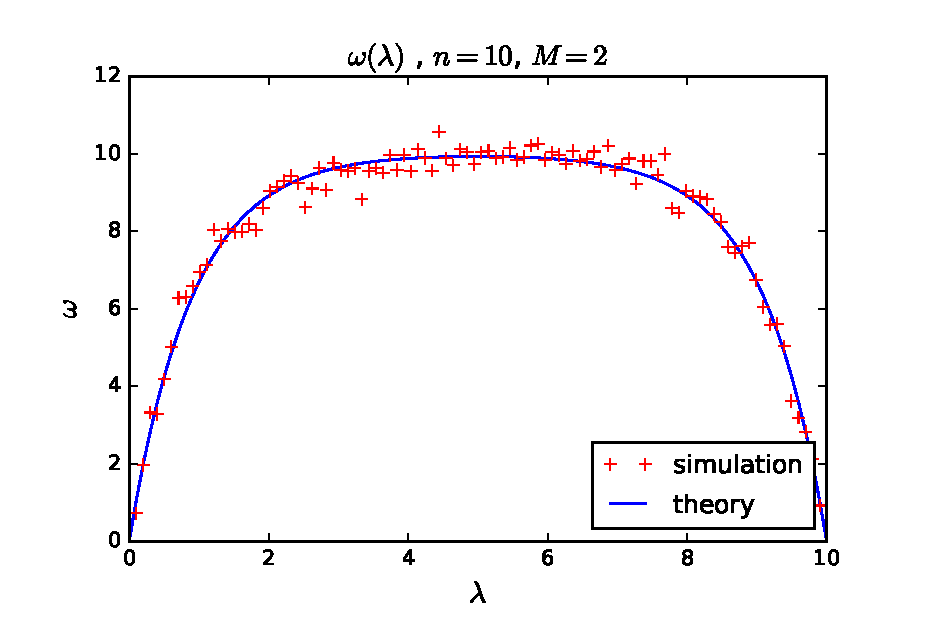
\includegraphics[height=3in]{wl_n10_m2}
\end{figure}
\end{frame}

\begin{frame}
\begin{figure}[b]
\centering
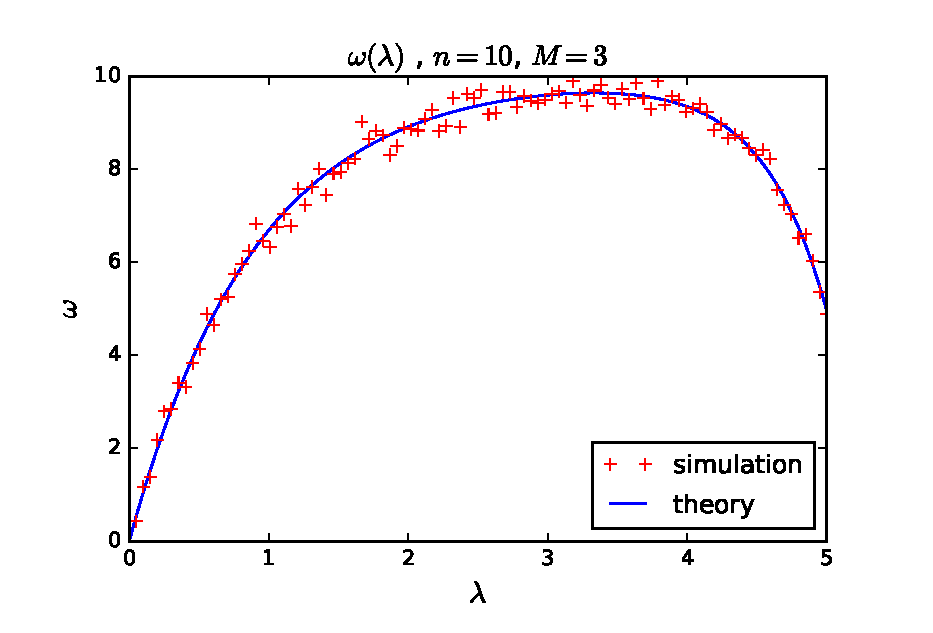
\includegraphics[height=3in]{wl_n10_m3}
\end{figure}
\end{frame}

\begin{frame}
\begin{figure}[b]
\centering
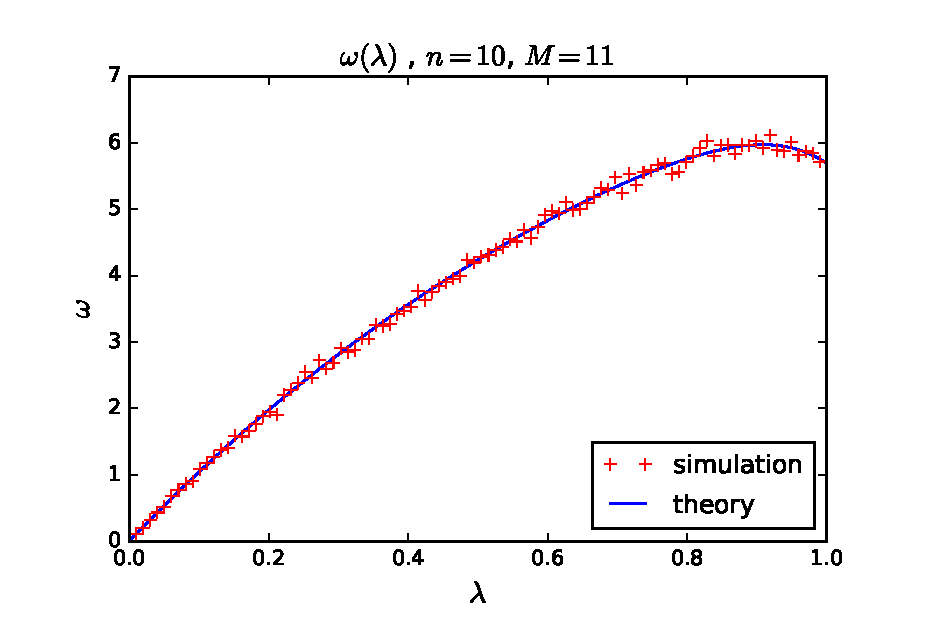
\includegraphics[height=3in]{wl_n10_m11}
\end{figure}
\end{frame}

\begin{frame}
\begin{figure}[b]
\centering
\includegraphics[height=3in]{wl_n40_m5}
\end{figure}
\end{frame}

\begin{frame}
\begin{figure}[b]
\centering
\includegraphics[height=3in]{p_nonzero_n10_m2}
\end{figure}
\end{frame}

\begin{frame}
\begin{figure}[b]
\centering
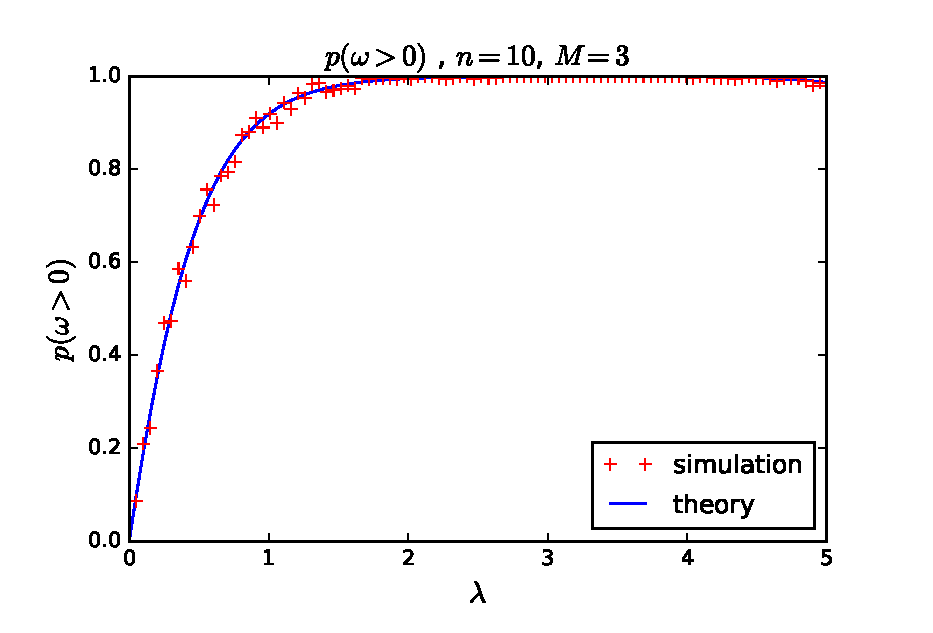
\includegraphics[height=3in]{p_nonzero_n10_m3}
\end{figure}
\end{frame}

\begin{frame}
\begin{figure}[b]
\centering
\includegraphics[height=3in]{p_nonzero_n10_m11}
\end{figure}
\end{frame}

\begin{frame}
\begin{figure}[b]
\centering
\includegraphics[height=3in]{p_nonzero_n40_m5}
\end{figure}
\end{frame}


\end{document}
